% ─── Slide: INT8 results ──────────────────────────────────────────────────────
\begin{frame}{INT8: Propagated Calibration Fixes the Real Problem}
  \begin{columns}[T]
    \begin{column}{0.46\textwidth}
      \textbf{Two ideas for closing the $10 \to 29$ gap:}

      \begin{enumerate}
        \item \textbf{Bin-centre loss} $\cos^2(\pi z)$:\\
          nudge $y_\mathrm{int}$ toward bin centres.\\
          \textit{Result: no improvement.}

        \vspace{0.5em}
        \item \textbf{Propagated calibration}:\\
          train layer $i$ on \emph{ADC-quantised} inputs from layer $i-1$\\
          (not clean FP inputs).\\
          \textit{Result: $-47\%$ ADC PPL.}
      \end{enumerate}

      \vspace{0.8em}
      \begin{alertblock}{Why propagation works}
        Standard layer-wise PTQ with FP inputs \emph{underestimates}
        the reconstruction difficulty at inference, where upstream ADC
        errors accumulate across layers.
      \end{alertblock}

      \vspace{0.5em}
      \begin{center}
      \small
      \begin{tabular}{lcc}
        \toprule
        Method & $\bypass$ & $\adcppl$ \\
        \midrule
        baseline       & 10.01 & 28.86 \\
        center         & 10.01 & 28.86 \\
        prop           & 11.01 & \better{14.55} \\
        \textbf{prop+center} & 11.00 & \best{14.41} \\
        \bottomrule
      \end{tabular}
      \end{center}
    \end{column}
    \begin{column}{0.50\textwidth}
      % plot_int8_main_results.pdf
      \iffalse
        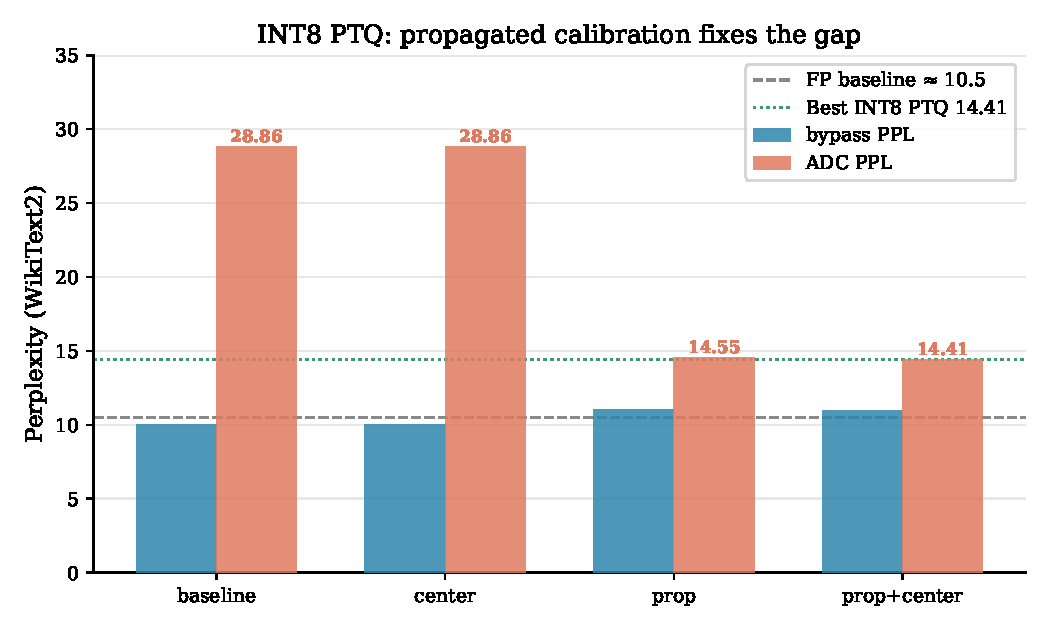
\includegraphics[width=\linewidth]{figs/plot_int8_main_results.pdf}
      \else
        \figplaceholder[0.65\textheight]{Grouped bar chart (4 methods on x-axis).
          Two bars per group: bypass PPL (light) and ADC PPL (dark).
          Highlight: center $\approx$ baseline; prop drops ADC PPL from 28.86 to 14.55;
          prop+center is marginal gain (14.41).
          Add FP baseline dashed line at 10.5.}
      \fi
    \end{column}
  \end{columns}
\end{frame}
